\documentclass[bwprint, withoutpreface]{cumcmthesis}

\usepackage{extarrows}
\usepackage{authblk}
\usepackage{tikz}
\usepackage{xcolor}
\usetikzlibrary{intersections, calc, bending, decorations.markings, arrows, shapes, positioning, decorations.pathreplacing}

\title{实变第三章总结}

\begin{document}
\maketitle
\noindent Author: Tony Xiang

\noindent Full Document can be acquired here: 

\noindent https://github.com/T0nyX1ang/RealAnaly-Documents/blob/master/Chapter\%203/Chapter3.pdf

\noindent Full Source code can be downloaded here:

\noindent https://github.com/T0nyX1ang/RealAnaly-Documents/blob/master/Chapter\%203/Chapter3.tex

\section{关于无穷的运算}
\indent $a \in \mathbb{R}^1$,则:
\begin{itemize}[itemindent=2em]
	\item 序关系:$-\infty < a < +\infty$.
	\item 加法:$a + (\pm{\infty}) = (\pm{\infty}) + a = (\pm{\infty}) + (\pm{\infty}) = (\pm{\infty})$.
	\item 减法:$a - (\mp{\infty}) = (\pm{\infty}) - (\mp{\infty}) = (\pm{\infty})$.
	\item 乘法:
	\begin{equation*}
	a \cdot (\pm{\infty}) = (\pm{\infty}) \cdot a = 
	\begin{cases}
		(\pm{\infty}), \quad 0 < a < +\infty \\
		0, \quad a = 0 \\
		(\mp{\infty}), \quad -\infty < a < 0
	\end{cases} 
	\end{equation*}.
	\item 除法:$\frac{a}{\pm{\infty}} = 0$.
	\item 绝对值:$|\pm{\infty}| = +\infty$.
	\item 未定义:$(\pm{\infty}) - (\pm{\infty})$,$\frac{\pm{\infty}}{\pm{\infty}}$,应避免出现.
\end{itemize}

函数,实值函数.

以下设$E \in \mathcal{M}(\mathbb{R}^n)$.

\section{可测函数的性质}
\indent 可测集:$E \in \mathcal{M}(\mathbb{R}^n)$,$f$为定义在$E$上的函数,若$\forall a \in \mathbb{R}^1$,$\{x \in E: f(x) > a\} \in \mathcal{M}(\mathbb{R}^n)$,称$f$为定义在$E$上的Lebesgue可测函数.

可测函数的示例:
\begin{itemize}[itemindent=2em]
	\item 常值函数是可测函数.
	\item $\chi_A$是可测函数$\Leftrightarrow$$A$是可测函数.特别地,Dirichlet函数为可测函数.
	\item 连续函数为可测函数,这说明一个函数的可测性条件并不算强.证明使用了$\{x \in E: f(x) > a\} = E \cap G$,$G$为开集的结论.
	\item $[a, b]$上的单调函数为可测函数,证明将检验的集合分为区间,单点集和空集三类处理.
\end{itemize}

可测函数的基本性质:
\begin{itemize}[itemindent=2em]
	\item $f$在$E$上可测,$E_1$是$E$的可测子集,则$f$在$E_1$上可测.证明使用:
	\begin{equation*}
		\{x \in E_1: f(x) > a\} = \{x \in E: f(x) > a\} \cap E_1
	\end{equation*}
	\item $E_1, E_2$是$E$的可测子集,$E = E_1 \cup E_2$,$f$在$E_1$上可测,$f$在$E_2$上可测,则$f$在$E$上可测.证明使用:
	\begin{equation*}
		\{x \in E: f(x) > a\} = \{x \in E_1: f(x) > a\} \cup \{x \in E_2: f(x) > a\}
	\end{equation*} 
\end{itemize}

简记符号:$\{x \in E: f(x) > a\} \to E(f > a)$.

\textbf{可测函数(TFAE):}
\begin{itemize}[itemindent=2em]
	\item $f$是$E$上的可测函数.
	\item $\forall a \in \mathbb{R}^1, E(f \geqslant a) \in \mathcal{M}(\mathbb{R}^n)$.
	\item $\forall a \in \mathbb{R}^1, E(f < a) \in \mathcal{M}(\mathbb{R}^n)$.
	\item $\forall a \in \mathbb{R}^1, E(f \leqslant a) \in \mathcal{M}(\mathbb{R}^n)$.
	\item $\forall A \in \mathcal{B}(\mathbb{R}^n), f^{-1}(A) \in \mathcal{M}(\mathbb{R}^n), E(f = +\infty) \in \mathcal{M}(\mathbb{R}^n)$
\end{itemize}

前四条互相证明可以由集合的运算来完成:
\begin{align*}
	& E(f \geqslant a) = \bigcap_{k = 1}^{\infty}{E(f > a - \frac{1}{k})} \\
	& E(f < a) = E - E(f \geqslant a) \\
	& E(f \leqslant a) = \bigcap_{k = 1}^{\infty}{E(f < a + \frac{1}{k})} \\
	& E(f > a) = E - E(f \leqslant a)
\end{align*}

第一条与第五条的互相证明:从左至右仅需了解即可,从右至左使用:
\begin{align*}
	& E(f = +\infty) = \bigcap_{k = 1}^{\infty}{E(f > k)} \\
	& E(f > a) = E(a < f \leqslant +\infty) = f^{-1}((a, +\infty)) \cup E(f = +\infty)
\end{align*}

注:$E(a < f < b), E(a \leqslant f < b), E(a < f < \leqslant b), E(a \leqslant f \leqslant b), E(f = -\infty)$均是可测集.

\textbf{可测函数的运算封闭性:}

注:规定若$f(x), g(x)$在某一点$x$处取异号的$\infty$为值,则规定$f(x) + g(x) = 0$.

\begin{itemize}[itemindent=2em]
	\item (对数乘的封闭性)$f$在$E$上可测,$c \in \mathbb{R}^1$,则$cf$在$E$上可测.证明使用下面的集合分解:
	\begin{equation*}
	E(cf > a) = 
	\begin{cases}
		E(f > \frac{a}{c}), \quad c > 0 \\
		E(f < \frac{a}{c}), \quad c < 0 \\
		E(0 > a), \quad c = 0
	\end{cases}
	\end{equation*}
	\item (对加法的封闭性)$f, g$在$E$上可测,则$f+g$在$E$上可测.证明先对有限情形使用\textbf{有理数的稠密性和有理数集的可列性质}:
	\begin{align*}
		& f(x) + g(x) > a \Leftrightarrow \exists r_n \in \mathbb{Q}^n, (f(x) > r_n) \wedge (g(x) > a - r_n) \\
		& E(f + g > a) = \bigcup_{k = 1}^{\infty}{(E(f > r_n) \cap E(g > a - r_n))}
	\end{align*}
	\indent 再考虑无限情况:
	\begin{align*}
		& A = (E(f = +\infty) \cap E(g = -\infty)) \cup (E(f = -\infty) \cap E(g = +\infty)) \\
		& E(f + g > a) = \{x \in E - A: f(x) + g(x) > a\} \cup \{x \in A: f(x) + g(x) > a\}
	\end{align*}
	\item (对乘法的封闭性)$f, g$在$E$上可测,则$fg$在$E$上可测.证明分两步,先证明$f^2$在$E$上可测,再得出题目结论.
	\begin{equation*}
	E(f^2 > a) = 
	\begin{cases}
		E, \quad a < 0 \\ 
		E(f > \sqrt{a}) \cup E(f < \sqrt{a}), \quad a \geqslant 0
	\end{cases}
	\end{equation*}
	\begin{equation*}
		2fg = (f + g)^2 - (f^2 + g^2)
	\end{equation*}
	\item (对绝对值的封闭性)$f$在$E$上可测,则$|f|$在$E$上可测.证明使用下面的集合分解:
	\begin{equation*}
	E(|f| > a) = 
	\begin{cases}
		E, \quad a < 0 \\
		E(f > a) \cup E(f < -a), \quad a \geqslant 0
	\end{cases}
	\end{equation*}
\end{itemize}

函数的正部与负部:$f^{+}(x) = \max\{f(x), 0\}, f^{-}(x) = \max\{-f(x), 0\}$.

正部与负部的性质:
\begin{itemize}[itemindent=2em]
	\item (非负性)$f^{+}(x) \geqslant 0, f^{-}(x) \geqslant 0$.
	\item (计算公式)$f(x) = f^{+}(x) - f^{-}(x), |f(x)| = f^{+}(x) + f^{-}(x)$.
	\item (可测性)$f^{+}(x), f^{-}(x)$在$E$上可测.证明可以用集合分解来处理.
	\begin{align*}
	& E(f^{+} > a) = 
	\begin{cases}
		E(f > a), \quad a \geqslant 0 \\
		E, \quad a < 0
	\end{cases} \\
	& E(f^{-} > a) = 
	\begin{cases}
		E(f < -a), \quad a \geqslant 0 \\
		E, \quad a < 0
	\end{cases}
	\end{align*}
\end{itemize}

注意:引入正部与负部的原因是方便之后对积分的处理,即先考虑非负值.

可测函数列的性质:$\{f_n\}$是$E$上的可测函数列,则函数\[\sup_{n \geqslant 1}{f_n}, \inf_{n \geqslant 1}{f_n}, \varlimsup_{n \to \infty}{f_n}, \varliminf_{n \to \infty}{f_n} \mbox{在$E$上可测.} \]

特别地,$\forall x \in E$, \[\lim_{n \to \infty}{f_n(x)} \mbox{存在,则其在$E$上可测.} \]证明可以用集合分解来处理:
\begin{align*}
	& E(\sup_{n \geqslant 1}{f_n} > a) = \bigcup_{n = 1}^{\infty}{E(f_n > a)} \\
	& E(\inf_{n \geqslant 1}{f_n} < a) = \bigcup_{n = 1}^{\infty}{E(f_n < a)} \\
	& \varlimsup_{n \to \infty}{f_n(x)} = \inf_{n \geqslant 1} \sup_{k \geqslant n}{f_k(x)} \\
	& \varliminf_{n \to \infty}{f_n(x)} = \sup_{n \geqslant 1} \inf_{k \geqslant n}{f_k(x)}
\end{align*}

可测分割:设$E \in \mathcal{M}(\mathbb{R}^n)$,$A_1, A_2, \cdots, A_k$是$E$的互不相交的可测子集,且$\bigcup_{i = 1}^{k}{A_i}$,则称$\{A_1, A_2, \cdots, A_k\}$是$E$的一个可测分割.

\textbf{简单函数:}$f$是定义在$E$上的函数,若存在$E$的一个可测分割$\{A_1, A_2, \cdots, A_k\}$与实数$a_1,a_2,\cdots,a_n$,使得$x \in A_i, f(x) = a_i(i = 1, 2, \cdots, k)$,则称$f$是定义在$E$上的简单函数.

\begin{equation*}
	f \mbox{是$E$上的简单函数} \Leftrightarrow f(x) = \sum_{i = 1}^{k}{a_i \chi_{A_i}(x), x \in E}
\end{equation*}

简单函数的性质:
\begin{itemize}[itemindent=2em]
	\item (对数乘的封闭性)$f$是简单函数,则$cf$是简单函数.证明将系数更改即可.
	\item (对加法的封闭性)$f, g$是简单函数,则$f + g$是简单函数.证明时写出$E$的两个可测分割,做出$\{A_i \cap B_j\}$亦为$E$的可测分割,并有$f(x) + g(x) = a_i + b_j, x \in A_i \cap B_j$. 注意,这说明给定两个简单函数,\textbf{可以设它们的表达式中所对应的$E$的可测分割是一样的.}
	\item (复合运算的性质)$\varphi$是$\mathbb{R}^1$上的\textbf{实值函数},则$\varphi(f(x))$是简单函数.证明直接写出$\varphi(f(x)) = \sum_{i = 1}^{k}{\varphi(a_i)\chi_{A_i}(x)}$.
\end{itemize}

函数列的单调性(仅说明单调增加性):$\{f_n\}$是$E$上的一列非负可测函数,$\forall x \in E, f_1(x) \leqslant f_2(x) \leqslant \cdots \leqslant f_n(x) \leqslant f_{n + 1}(x) \leqslant \cdots$,则称函数列$\{f_n\}$是单调增加的.记为$\{f_n\} \nearrow$.

逼近定理:设$f$是E上的非负可测函数,则存在$E$上的单调增加的非负简单函数列$\{f_n\}$,使得$\{f_n\} \nearrow f(n \to \infty)$.若$f$在$E$上是有界的,则$f_n \rightrightarrows f$.(证明略)

逼近定理的推论:设$f$是$E$上的非负可测函数,则存在$E$上的非负简单函数列$\{f_n\}$,使得$\{f_n\} \to f(n \to \infty), |f_n| \leqslant |f|(n \geqslant 1)$.若$f$在$E$上是有界的,则$f_n \rightrightarrows f$.证明可以将$f$分为正部与负部分别处理然后合并.

\textbf{可测函数的构造性特征:}$f$是E上的函数,则$f\mbox{可测}\Leftrightarrow \exists \mbox{简单函数列} \{f_n\}, s.t. \{f_n(x)\} \to f(x) (x \in E, n \to \infty)$.

复合函数的可测性:$f$是$E$上的实值可测函数,$g$是$\mathbb{R}^1$上的连续函数,则$g(f(x))$在$E$上可测.使用可测函数的构造性特征证明.

\section{可测函数列的收敛}

\indent 几乎处处成立的性质:$m(\{x \in E: \neg P(x)\}) = 0$,或$\exists E_0 \subset E, m(E_0) = 0, s.t. \quad x \in E - E_0, P(x)$.则称$P(x)$在$E$上几乎处处成立,记为$P(x) a.e. \mbox{于} E$.

几乎处处成立的示例:
\begin{itemize}[itemindent=2em]
	\item 几乎处处相等:$f, g$为$E$上的函数,$m(E(f \neq g)) = 0$,则$f = g, a.e.\mbox{于}E$.
	\item 几乎处处有限:$f$为$E$上的函数,$m(E(|f| = \infty)) = 0$,则$f$在$E$上几乎处处有限.
	\item 本性有界:$f$为$E$上的函数,$\exists M > 0, m(E(|f| > M)) = 0$,则$f$在$E$上本性有界.
\end{itemize}   

\textbf{注意几乎处处有限与本性有界的区别,本性有界的结论更强.}

$f$在$E$上可测,$f = g, a.e.\mbox{于}E$,则$g$在$E$上可测.即改变函数在一个零测集上的函数值,不改变函数的可测性.证明使用以下的集合分解:
\begin{align*}
	E(g > a) & = {\{x \in E - E_0: g(x) > a} \cup {x \in E_0: g(x) > a\}} \\
			 & = {\{x \in E - E_0: f(x) > a} \cup {x \in E_0: g(x) > a\}}
\end{align*}

\textbf{可测函数的几种收敛:}
\begin{itemize}[itemindent=2em]
	\item 几乎处处收敛:$\exists E_0 \subset E, m(E_0) = 0, s.t. \quad x \in E - E_0, f_n(x) \to f(x)$,记为$f_n \to f \quad a.e. \mbox{于}E$.
	\item 依测度收敛:$\forall \varepsilon > 0, \lim_{n \to \infty}{m(E(|f_n(x) - f(x)| \geqslant \varepsilon))} = 0$,记为$f_n \stackrel{m}{\longrightarrow} f\mbox{于}E$.
	\item 几乎一致收敛:$\forall \delta > 0, \exists E_{\delta} \subset E, m(E - E_{\delta}) < \delta, s.t. \quad f_n(x) \rightrightarrows f(x), x \in E_{\delta}$,$f_n \to f \quad a.un. \mbox{于}E$.
\end{itemize}

注意:依测度收敛是从整体的角度反映当$n \to \infty$时$\{f_n\}$的变化性态的一种收敛.

\textbf{几种收敛的相互关系:}
\begin{center}
\begin{tikzpicture}[decoration={markings,mark=at position 0.52 with {\arrow{stealth}}}]
	\coordinate (ae) at (90:3cm);
	\coordinate (aun) at (210:3cm);
	\coordinate (am) at (-30:3cm);
	\node[above] at (ae) {几乎处处收敛};
	\node[below left] at (aun) {几乎一致收敛};
	\node[below right] at (am) {依测度收敛};
	\fill[black, opacity=0.8] (ae) circle (2pt);
	\fill[black, opacity=0.8] (am) circle (2pt);
	\fill[black, opacity=0.8] (aun) circle (2pt);
	\draw [postaction={decorate}, thick, black] (ae.south) to [bend right=15] (am.north east);
	\draw [postaction={decorate}, thick, black] (am.north east) to [bend right=15] (ae.south);
	\draw [postaction={decorate}, thick, black] (aun.east) -- (am.west);
	\draw [postaction={decorate}, thick, black] (ae.north east) to [bend right=15] (aun.south);
	\draw [postaction={decorate}, thick, black] (aun.north east) to [bend right=15] (ae.south);
	\node [left, align=justify, font=\small] at (150:2.3cm) {$m(E) < \infty$ \\ Egoroff thm.};
	\node [right, align=justify, font=\small] at (30:2.3cm) {$\exists \{f_{n_k}\} \subset \{f_n\}$ \\ Risez thm.};
	\node [below, align=justify, font=\small] at (-25:1.0cm) {$m(E) < \infty$};
\end{tikzpicture}
\end{center}

\textbf{Risez定理的一个应用:}$m(E) < \infty$,则:
\begin{equation*}
	f_n \stackrel{m}{\longrightarrow} f \Leftrightarrow \forall \{f_{n_k}\} \subset \{f_n\}, \exists \{f_{n_{k'}}\} \subset \{f_{n_k}\}, s.t. \quad f_{n_{k'}} \to f \quad a.e.
\end{equation*}

\textbf{注意:我们期望将依测度收敛转化为几乎处处收敛,因为依测度收敛的形式较为复杂,而几乎处处收敛可以转化为数列的极限来处理,这样就大大地减少了分析的难度.}

部分定理的证明写在附录中.

\section{可测函数与连续函数的关系}

Lusin定理的引理:设$F_1, F_2, \cdots, F_k$是$\mathbb{R}^n$中的$k$个互不相交的闭集,$F = \bigcup_{i = 1}^{k}{F_i}$,则简单函数$f(x) = \sum_{k = 1}^{k}{a_i \chi_{F_i}(x)}$是$F$上的连续函数.可以直接按连续性的定义证明:$\delta = d(x_0, \bigcup_{i \neq i_0}{F_i}), x_0 \in \bigcup_{i \neq i_0}{F_i}$.

Lusin定理:设$E$是$\mathbb{R}^n$中的可测集,$f$是$E$上$a.e.$有限的可测函数,则$\forall \delta > 0, \exists F_{\delta} \subset E, F_{\delta}\mbox{为闭集}, s.t. \quad m(E - F_{\delta}) < \delta$,且$f$是$F_{\delta}$上的连续函数.

注意:此处的连续函数是限制在$F_{\delta}$上的连续函数,并不能保证原函数的连续性.

Tietze扩张定理:设$F$是$\mathbb{R}^n$中的闭集,$f \in C(F), \exists g \in C(\mathbb{R}^n), s.t. \quad x \in F, g(x) = f(x)$,且$\sup_{x \in \mathbb{R}^n}{|g(x)|} = \sup_{x \in F}{|f(x)|}$.(证明略)

Lusin定理的加强形式:设$E$是$\mathbb{R}^n$中的可测集,$f$是$E$上$a.e.$有限的可测函数,则$\forall \delta > 0, \exists g \in C(\mathbb{R}^n), s.t. \quad m(\{x \in E:f(x) \neq g(x)\}) < \delta$,且$f$是$F_{\delta}$上的连续函数.且$\sup_{x \in \mathbb{R}^n}{|g(x)|} = \sup_{x \in F}{|f(x)|}$.证明使用了原有的Lusin定理和Tietze扩张定理:
\begin{align*}
	& \sup_{x \in \mathbb{R}^n}{|g(x)|} \leqslant \sup_{x \in F}{|f(x)|} \leqslant \sup_{x \in E}{|f(x)|}. \\
	& \{x \in E:f(x) \neq g(x)\} \subset E - F \\
	& m(\{x \in E:f(x) \neq g(x)\}) \leqslant m(E - F) < \delta
\end{align*}

本节之后的内容不作要求,部分定理的证明写在附录中.

\appendix
\section{布置的课后作业}
\indent $1,2,3,4,5,6,7,8,9,11,13,14,15,16,17,18(1),19,20(3)(4),21,22,24,25,27.$

\section{课后作业的讲解}

\section{部分定理的证明与相关反例的构造}
\subsection{收敛关系的一些相互推导}
\begin{theorem}
	设$m(E) < \infty$,$f_n \to f \quad a.e.\mbox{于}E$,$\forall \varepsilon > 0,$
	\begin{equation*}
		\lim_{n \to \infty} m(\bigcup_{k = n}^{\infty}{E(|f_n - f| \geqslant \varepsilon)}) = 0.
	\end{equation*} 
\end{theorem}

\begin{proof}
	对于给定的$x_0 \in E$,若$\forall n \geqslant 1, \exists k \geqslant n, s.t. \quad |f_k(x_0) - f(x_0)| \geqslant \varepsilon$,则$f_k(x_0)$不收敛于$f(x_0)$,这表明:
	\begin{equation*}
		\bigcap_{n = 1}^{\infty}{\bigcup_{k = n}^{\infty}{E(|f_k - f| \geqslant \varepsilon)}} \subset \{x \in E: f_k(x) \nrightarrow f(x)\}.
	\end{equation*}
	由于$f_n \to f \quad a.e. \mbox{于}E$,上式右边的集为零测集,故
	\begin{equation*}
		m(\bigcap_{n = 1}^{\infty}{\bigcup_{k = n}^{\infty}{E(|f_k - f| \geqslant \varepsilon)}}) = 0.
	\end{equation*}
	而$m(E) < \infty$,由测度的上连续性,有
	\begin{equation*}
		\lim_{n \to \infty} m(\bigcup_{k = n}^{\infty}{E(|f_k * f| \geqslant \varepsilon)}) = m(\bigcap_{n = 1}^{\infty}{\bigcup_{k = n}^{\infty}{E(|f_k - f| \geqslant \varepsilon)}}) = 0.
	\end{equation*}
\end{proof}

\begin{theorem}[Egoroff定理]
	设$m(E) < \infty$,$f_n \to f \quad a.e.$,则$f_n \to f \quad a.un.$
\end{theorem}

\begin{proof}
	由\textbf{定理$1$},$\forall k \geqslant 1$,
	\begin{equation*}
		\lim_{n \to \infty}{m(\bigcup_{i = n}^{\infty}{E(|f_i - f| \geqslant \frac{1}{k})})} = 0.	
	\end{equation*}
	于是对任意给定的$\delta > 0$,可以依次选取自然数$k_1, k_2, \cdots, n_k, \cdots, s.t.$
	\begin{equation*}
		m(\bigcup_{i = n}^{\infty}{E(|f_i - f| \geqslant \frac{1}{k})}) < \frac{\delta}{2^k}, k = 1, 2, \cdots.
	\end{equation*}
	
	\textbf{令\[E_{\delta} = \bigcap_{k = 1}^{\infty}{\bigcup_{i = n_k}^{\infty}{E(|f_i - f| < \frac{1}{k})}}.\]}
	
	由De Morgan公式得,
	\begin{align*}
		E - E_{\delta} & = \bigcup_{k = 1}^{\infty}{\bigcup_{i = n_k}^{\infty}{E(|f_i - f| \geqslant \frac{1}{k})}} \\
		m(E - E_{\delta}) & = m(\bigcup_{k = 1}^{\infty}{\bigcup_{i = n_k}^{\infty}{E(|f_i - f| \geqslant \frac{1}{k})}}) \\
						  & \leqslant \sum_{k = 1}^{\infty}{m(\bigcup_{i = n_k}^{\infty}{E(|f_i - f| \geqslant \frac{1}{k})})} \\
						  & < \sum_{k = 1}^{\infty}{\frac{\delta}{2^k}} = \delta. 
	\end{align*}
	所以$\forall \varepsilon > 0, \exists k, s.t. \quad \frac{1}{k} < \varepsilon$.则当$i \geqslant n_k, \forall x \in E$,
	\begin{equation*}
		|f_i(x) - f(x)| < \frac{1}{k} < \varepsilon.
	\end{equation*}
	即$f_n \rightrightarrows f$于$E_{\delta}$,即$f_n \rightrightarrows f \quad a.un.\mbox{于}E$.
\end{proof}

\begin{theorem}
	设$m(E) < \infty$,若$f_n \to f \quad a.e.$,则$f_n \stackrel{m}{\longrightarrow} f$.
\end{theorem}

\begin{proof}
	由\textbf{定理$1$},$\forall \varepsilon > 0$,
	\begin{equation*}
		\lim_{n \to \infty}{m(\bigcup_{k = n}^{\infty}{E(|f_k - f| \geqslant \varepsilon)})} = 0.
	\end{equation*}
	则由测度单调性,
	\begin{equation*}
		0 \leqslant m(E(|f_n - f| \geqslant \varepsilon)) \leqslant m(\bigcup_{k = n}^{\infty}{E(|f_k - f| \geqslant \varepsilon)}).
	\end{equation*}
	令$n \to \infty$,得到\[\lim_{n \to \infty}{E(|f_n - f| \geqslant \varepsilon)} = 0 \mbox{,即} f_n \stackrel{m}{\longrightarrow} f.\]
\end{proof}

\begin{theorem}[Risez定理]
	若$f_n \stackrel{m}{\longrightarrow} f$,则$\exists \{f_{n_k}\} \subset \{f_n\}, s.t. \quad f_{n_k} \to f_n \quad a.e.$
\end{theorem}

\begin{proof}
	$f_n \stackrel{m}{\longrightarrow} f$,则$\forall \varepsilon > 0, \delta > 0, \exists n \geqslant 1, s.t. \quad n \geqslant N, m(E(|f_n - f| \geqslant \varepsilon)) < \delta$.
	于是$\forall k \in \mathbb{N}^*$,令$\varepsilon = \frac{1}{k}, \delta = \frac{1}{2^k}$,可以依次选取自然数$n_1, n_2, \cdots, n_k, \cdots, s.t.$
	\begin{equation*}
		m(E(|f_{n_k} - f| \geqslant \frac{1}{k})) < \frac{1}{2^k}.
	\end{equation*}
	下面证明$f_{n_k} \to f \quad a.e.$ \\
	\textbf{令\[E_0 = \bigcap_{N = 1}^{\infty}{\bigcup_{k = N}^{\infty}{E(|f_k - f| \geqslant \frac{1}{k})}}.\]}
	对每个$N = 1, 2, \cdots, $有
	\begin{equation*}
		m(E_0) \leqslant m(\bigcup_{k = N}^{\infty}{E(|f_{n_k} - f| \leqslant \frac{1}{k})}) \leqslant \sum_{k = N}^{\infty}{m(E(|f_{n_k} - f| \geqslant \frac{1}{k}))} < \sum_{k = N}^{\infty}{\frac{1}{2^k}} = \frac{1}{2^{N - 1}}.
	\end{equation*}
	令$N \to \infty$,可知$m(E_0) = 0$.
	由De Morgan公式得,
	\begin{equation*}
		E - E_0 = \bigcup_{N = 1}^{\infty}{\bigcap_{k = N}^{\infty}{E(|f_k - f| \geqslant \frac{1}{k})}}.
	\end{equation*}
	所以$\forall x \in E - E_0, \exists N \geqslant 1, s.t. \quad k \geqslant N$,
	\begin{equation*}
		|f_{n_k}(x) - f(x)| < \frac{1}{k}.
	\end{equation*}
	故$f_{n_k}(x) \to f(x)$,则在$E$上$f_{n_k} \to f \quad a.e.$
\end{proof}

\begin{theorem}[Risez定理的一个应用]
	\begin{equation*}
		f_n \stackrel{m}{\longrightarrow} f \Leftrightarrow \forall \{f_{n_k}\} \subset \{f_n\}, \exists \{f_{n_{k'}}\} \subset \{f_{n_k}\}, s.t. \quad f_{n_{k'}} \to f \quad a.e.		
	\end{equation*}
\end{theorem}

\begin{proof}
	($\Rightarrow$)设$f_n \stackrel{m}{\longrightarrow}f$,则$\forall \{f_{n_k}\} \subset \{f_n\}$,$f_{n_k} \stackrel{m}{\longrightarrow} f$(直接按照定义证明),由\textbf{定理$3$}(Risez定理),$\exists \{f_{n_{k'}}\} \subset \{f_{n_k}\}, s.t. \quad f_{n_{k'}} \to f \quad a.e. (k' \to \infty).$ \\
	($\Leftarrow$)用反证法,若$\{f_n\} \stackrel{m}{\nrightarrow} f$,$\exists \varepsilon > 0, s.t. \quad m(E(|f_n - f| \geqslant \varepsilon)) \nrightarrow 0$,于是$\exists \delta > 0, \{f_{n_k}\} \subset \{f_n\}, s.t.$ \[m(E(|f_{n_k} - f| \geqslant \varepsilon)) \geqslant \delta, \quad k = 1, 2, \cdots.\]另一方面,由假设条件,$\exists \{f_{n_{k'}}\} \subset \{f_{n_k}\}, s.t. \quad f_{n_{k'}} \to f \quad a.e.$ \\
	因为$m(E) < \infty$,由\textbf{定理$2$},$f_{n_{k'}} \stackrel{m}{\longrightarrow} f$,从而得出矛盾.从而$f_n \stackrel{m}{\longrightarrow} f$.
\end{proof}

\subsection{相关反例的构造}
\begin{example}[几乎处处收敛不能推出依测度收敛]
	$\forall n \in \mathbb{R}^*$,令
	\begin{equation*}
	f_n(x) = 
	\begin{cases}
		1, \quad x \in [0, n] \\
		0, \quad x \in (n, \infty).
	\end{cases}
	\end{equation*}
	$f_n \to 1, a.e. \mbox{于}[0, n)$,但$f_n \stackrel{m}{\nrightarrow} 1.$
\end{example}

\begin{example}[依测度收敛不能推出几乎处处收敛]
	$\forall n \in \mathbb{N}^*$,将区间$[0, 1]$分为$n$个等长的小区间,记
	\begin{equation*}
		A_n^i = [\frac{i - 1}{n}, \frac{i}{n}], i = 1, 2, \cdots, n.
	\end{equation*}
	将$\{A_n^i\}$按照下图所示的顺序$A_1^1, A_2^1, A_2^2, A_3^1, A_3^2, A_3^3, \cdots$重新编号记为$\{E_n\}$,显然$m(E_n) \to 0, n \to \infty$,令$f_n(x) = \chi_{E_n}(x), x \in [0, 1].$
	\begin{center}
		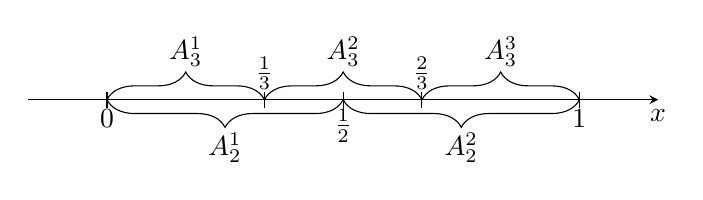
\begin{tikzpicture}
			\draw[-{stealth[black]}] (-1, 0) -- (7, 0);
			\foreach \x in {0, 2, 3, 4, 6}
				\draw (\x, -0.1) -- (\x, 0.1);
			\draw [decorate, decoration={brace, amplitude=10}] (0, 0) -- (2, 0);
			\draw [decorate, decoration={brace, amplitude=10}]  (2, 0) -- (4, 0);
			\draw [decorate, decoration={brace, amplitude=10}]  (4, 0) -- (6, 0);
			\draw [decorate, decoration={brace, amplitude=10}]  (3, 0) -- (0, 0);
			\draw [decorate, decoration={brace, amplitude=10}]  (6, 0) -- (3, 0);
			\node [above, align=justify] at (1, 0.3) {$A_3^1$};
			\node [above, align=justify] at (3, 0.3) {$A_3^2$};
			\node [above, align=justify] at (5, 0.3) {$A_3^3$};
			\node [below, align=justify] at (1.5, -0.3) {$A_2^1$};
			\node [below, align=justify] at (4.5, -0.3) {$A_2^2$};
			\node [above, align=justify] at (2, 0) {$\frac{1}{3}$};
			\node [above, align=justify] at (4, 0) {$\frac{2}{3}$};
			\node [below, align=justify] at (3, 0) {$\frac{1}{2}$};
			\node [below, align=justify] at (0, 0) {$0$};
			\node [below, align=justify] at (6, 0) {$1$};
			\node [below, align=justify] at (7, 0) {$x$};
		\end{tikzpicture}
	\end{center}
	对任意$\varepsilon > 0$,(不妨设$\varepsilon < 1$),由于$n \to \infty$,$m(E(|f_n| \geqslant \varepsilon)) = m(E_n) \to 0$.
	$f_n \stackrel{m}{\longrightarrow} 0, \mbox{于}[0, 1]$,但$\{f_n\}$在$[0, 1]$上处处不收敛.因为有无限个$n$使得$f_n(x_0) = 1$,又有无限个$n$使得$f_n(x_0) = 0$.
\end{example}

\subsection{Lusin定理}
\begin{theorem}[Lusin定理]
	设$E$是$\mathbb{R}^n$中的可测集,$f$是$E$上$a.e.$有限的可测函数,则$\forall \delta > 0, \exists F_{\delta} \subset E, F_{\delta}\mbox{为闭集}, s.t. \quad m(E - F_{\delta}) < \delta$,且$f$是$F_{\delta}$上的连续函数.
\end{theorem}

\begin{proof}
	分两步证明. \\
	\textbf{第$1$步}:先设$f$为简单函数,即
	\begin{equation*}
		f(x) = \sum_{i = 1}^{k}{a_i \chi_{E_i}(x)},
	\end{equation*}
	其中$E_1, E_2, \cdots, E_k$是$E$的一个可测分割.由可测集的逼近定理,$\forall \delta > 0, i = 1, 2, \cdots, k$,$\exists F_i \subset E_i$,$F_i$为闭集,使得
	\begin{equation*}
		m(E_i - F_i) < \frac{\delta}{2^k}, \quad i = 1, 2, \cdots, k.
	\end{equation*}
	\textbf{令\[F_{\delta} = \bigcup_{i = 1}^{k}{F_i}\]},则$F_{\delta}$是$E$的闭子集,且
	\begin{equation*}
		m(E - F_{\delta}) = m(\bigcup_{i = 1}^{k}{(E_i - F_i)}) = \sum_{i = 1}^{k}{m(E_i - F_i)} < \delta.
	\end{equation*}
	\begin{equation*}
		f(x)|_{F_{\delta}} = \sum_{i = 1}^{k}{a_i \chi_{F_i}(x)} \mbox{,且$f \in C(F_{\delta})$}.
	\end{equation*}
	\textbf{第$2$步}:一般情形.设$f$是$E$上a.e.有限的可测函数.由于$E(|f| = \infty) = 0$,记之为$E_0$,则这个零测集不会影响$m(E - F_{\delta}) < \delta$.所以我们可以设$f$是处处有限的.若令
	\begin{equation*}
		g(x) = \frac{f(x)}{1 + |f(x)|} \mbox{,逆变换为:} f(x) = \frac{g(x)}{1 - |g(x)|}.
	\end{equation*}
	则$g$是有界可测函数,并且若$g \in C(F_{\delta})$,$f \in C(F_{\delta})$.故不妨设$f$有界.则由\textbf{第$1$步}的结论可知$\exists \{f_k\}, f_k \rightrightarrows f \mbox{于}E$.$\forall \delta > 0, \forall f_k, \exists F_k \subset E$,$F_k$为闭集,s.t. $f_k \in C(F_k)$,且$m(F - F_k) < \frac{\delta}{2^k}$. \\
	\textbf{令\[F_{\delta} = \bigcap_{i = 1}^{k}{F_i},\]}则$F_{\delta}$是$E$的闭子集,且
	\begin{equation*}
		m(E - F_{\delta}) = m(\bigcup_{k = 1}^{\infty}{E - F_k}) \leqslant \sum_{k = 1}^{\infty}{m(E - F_k)} < \delta.
	\end{equation*}
	由于$f_k \in C(F_{\delta})$,且$f_k \rightrightarrows f \mbox{于}F_{\delta}$.所以$f|_{F_{\delta}} \in C(F_{\delta})$.
\end{proof}

\end{document}